\begin{frame}
   \frametitle{Part 2: Reusing Computation Between Steps}
      \begin{tikzpicture}
      \draw[step=1,black!15,very thin,opacity=\gridopacity] (0,0) grid (12,8);
   
      % figure adapted from proposal doc
      \begin{scope}[font=\scriptsize,shift={(1.5,6.25)}]
         
         % root sets
         \node[draw,black,rounded corners,minimum height=1.5cm,minimum width=1cm]
            (Xgrasp) at (3,0) {};
         \node[above=0cm of Xgrasp] {Grasp};
         \node[draw,black,rounded corners,minimum height=1.5cm,minimum width=1cm]
            (Xdrop) at (6,0) {};
         \node[above=0cm of Xdrop] {Place};
         
         % nodes
         \node[circle,fill=black,inner sep=2] (xstart) at (0,0) {};
         \node[above=0.1cm of xstart] {$q_{\mbox{\scriptsize start}}$};
         
         % grasp choices
         \node[circle,fill=black,inner sep=2] (xg1) at (2.8,0.5) {};
         \node[circle,fill=black,inner sep=2] (xg2) at (3.1,0.1) {};
         \node[circle,fill=black,inner sep=2] (xg3) at (2.9,-0.5) {};
         % place choices
         \node[circle,fill=black,inner sep=2] (xd1) at (5.9,0.3) {};
         \node[circle,fill=black,inner sep=2] (xd2) at (6.0,-0.4) {};
         % xend 
         \node[circle,fill=black,inner sep=2] (xend) at (9,0) {};
         \node[above=0.1cm of xend] {$q_{\mbox{\scriptsize end}}$};
         
         \draw[line width=1.5mm,white]
            (xstart) .. controls (1,0.2) and (1.4,0.9) .. (xg1);
         \draw[line width=1.5mm,white]
            (xstart) .. controls (1.5,0.2) .. (xg2);
         \draw[line width=1.5mm,white]
            (xstart) .. controls (1.8,-0.6) and (1.6,-0.8) .. (xg3);
         \draw
            (xstart) .. controls (1,0.2) and (1.4,0.9) .. (xg1);
         \draw
            (xstart) .. controls (1.5,0.2) .. (xg2);
         \draw
            (xstart) .. controls (1.8,-0.6) and (1.6,-0.8) .. (xg3);
         \draw[line width=1.5mm,white]
            (xg1) -- (4.7,0.6);
         \draw
            (xg1) -- (4.7,0.6);
         \draw[line width=1.5mm,white]
            (xg2) .. controls (4.5,1) and (3.5,-1.2) .. (4.5,-0.4)
                  .. controls (5.5,0.5) and (5.0,-1.3) .. (xd2);
         \draw
            (xg2) .. controls (4.5,1) and (3.5,-1.2) .. (4.5,-0.4)
                  .. controls (5.5,0.5) and (5.0,-1.3) .. (xd2);
         \draw[line width=1.5mm,white]
            (xg3) .. controls (4.3, 0.2) and (4.5,-0.2) .. (xd1);
         \draw
            (xg3) .. controls (4.3, 0.2) and (4.5,-0.2) .. (xd1);
         % in s3
         \draw[line width=1.5mm,white]
            (xd1) .. controls (8,0.3) and (8,0.1) .. (xend);
         \draw
            (xd1) .. controls (8,0.3) and (8,0.1) .. (xend);
         
         \node[fill,black,rounded corners,minimum height=1.5cm,minimum width=1cm,
            opacity=0.1] at (3,0) {};
         \node[fill,black,rounded corners,minimum height=1.5cm,minimum width=1cm,
            opacity=0.1] at (6,0) {};
         
      \end{scope}
   
      \fill[green!20] (0.1,3.1) rectangle (11.9,3.7);
   
      \node[anchor=north] at (6,5) {\begin{minipage}{11.5cm}
         Planning for manipulation tasks poses three challenges:
         
         \begin{itemize}
         \item Challenge 1: Capturing the planning/execution tradeoff..
         \item Challenge 2: Incongruent steps impede reuse.
         \item Challenge 3: Coupled steps require long planning horizons.
         \end{itemize}
      \end{minipage}};
   
   \end{tikzpicture}
\end{frame}

\begin{frame}
   \frametitle{Motivation: Structure of Manipulation Problems}
   
   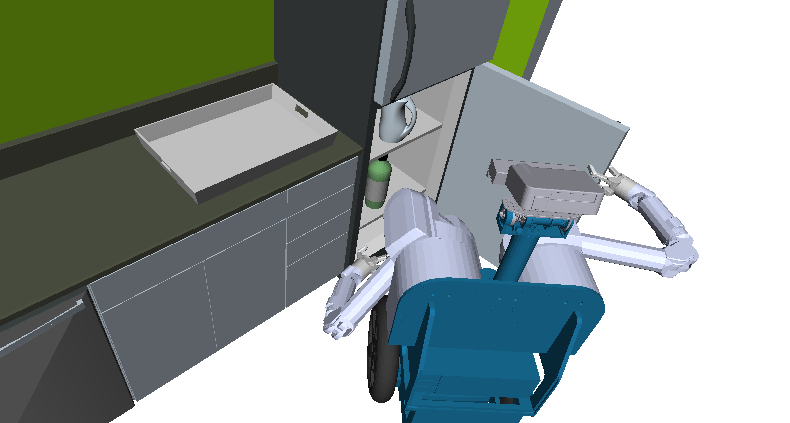
\includegraphics[width=\textwidth]{figs/fridge-intro.png}
   
\end{frame}

\begin{frame}
   \frametitle{Motivation: 2D Example}
   \begin{tikzpicture}

      \draw[step=1,black!15,very thin,opacity=\gridopacity] (0,0) grid (12,8);
      
      \node[inner sep=0] at (5.5,4.75) {
         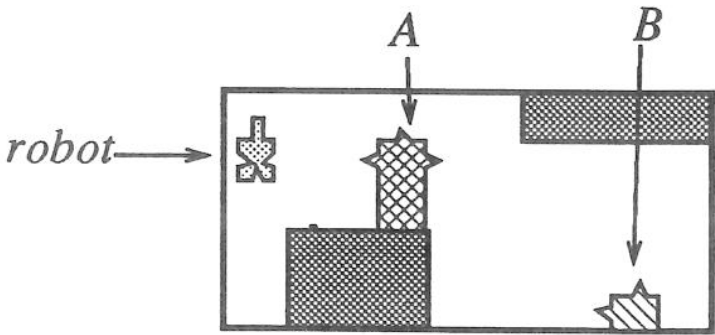
\includegraphics[width=5cm]{figs/alami-intro.png}
      };
      
      \node[inner sep=0pt] at (6,0.5) {\begin{minipage}{7.75cm}\scriptsize{
         $^\dag$\PaperPortrait\;  Alami, Simeon, and Laumond,
         ``A Geometrical Approach to Planning Manipulation Tasks,'' ISRR 1990.
      }\end{minipage}};
      
   \end{tikzpicture}
\end{frame}


\begin{frame}
   \frametitle{Motivation: 2D Example}
   \begin{tikzpicture}
   
      \draw[step=1,black!15,very thin,opacity=\gridopacity] (0,0) grid (12,8);
      
      \node[inner sep=0] at (5.5,6.75) {
         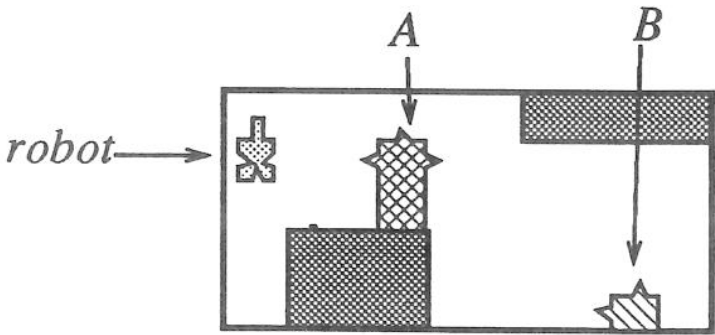
\includegraphics[width=5cm]{figs/alami-intro.png}
      };
      
      \node[inner sep=0] at (0.75,4.25) {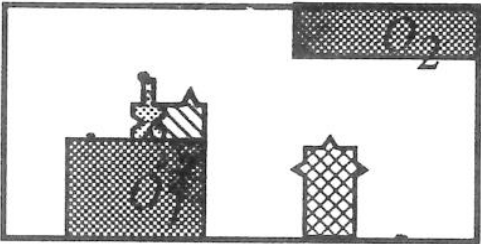
\includegraphics[width=1cm]{figs/alami-transit-1.png}};
      \node[inner sep=0] at (0.75,3.6) {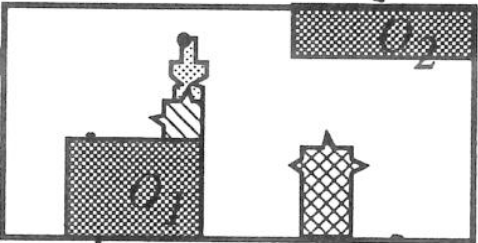
\includegraphics[width=1cm]{figs/alami-intersection.png}};
      \node[inner sep=0] at (0.75,2.95) {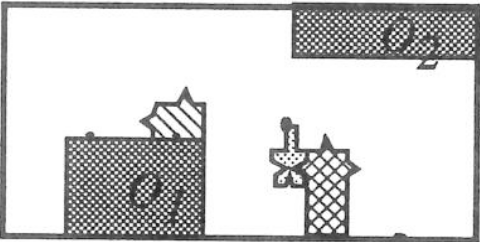
\includegraphics[width=1cm]{figs/alami-transit-4.png}};
      \node[inner sep=0] at (0.75,2.3) {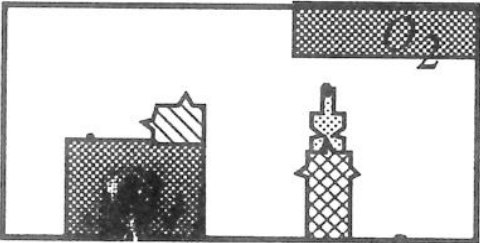
\includegraphics[width=1cm]{figs/alami-transit-3.png}};
      \node[inner sep=0] at (0.75,1.65) {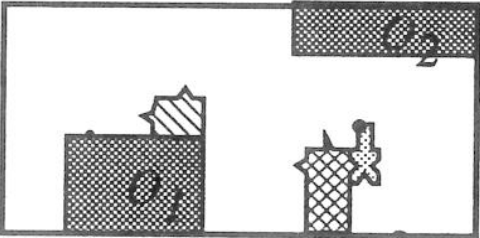
\includegraphics[width=1cm]{figs/alami-transit-2.png}};
      
      \node at (3.25,4.9) {Transit Slice:};
      \node[inner sep=0] at (3.5,3.5) {%
         \only<1>{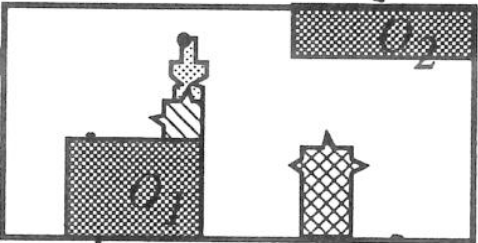
\includegraphics[width=4cm]{figs/alami-intersection.png}}%
         \only<2>{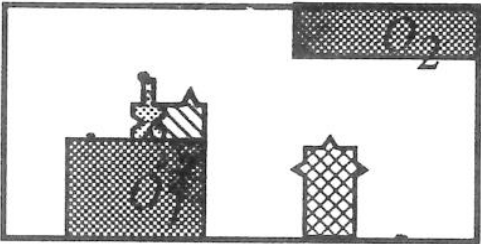
\includegraphics[width=4cm]{figs/alami-transit-1.png}}%
         \only<3>{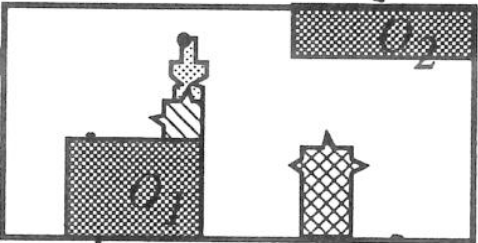
\includegraphics[width=4cm]{figs/alami-intersection.png}}%
         \only<4>{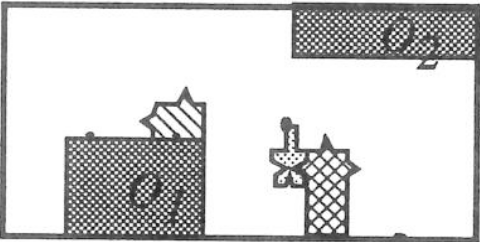
\includegraphics[width=4cm]{figs/alami-transit-4.png}}%
         \only<5>{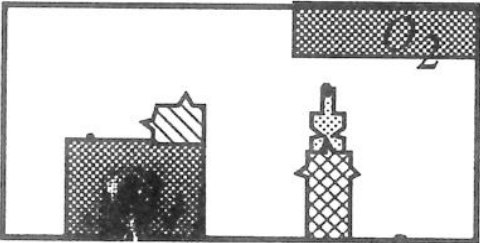
\includegraphics[width=4cm]{figs/alami-transit-3.png}}%
         \only<6>{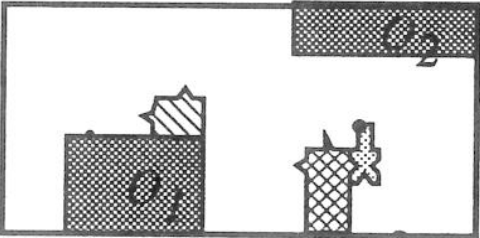
\includegraphics[width=4cm]{figs/alami-transit-2.png}}%
         \only<7->{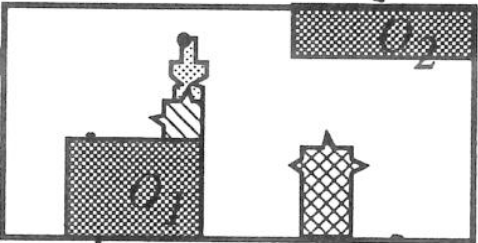
\includegraphics[width=4cm]{figs/alami-intersection.png}}%
      };
      \node[inner sep=0] at (3.5,1.25) {
         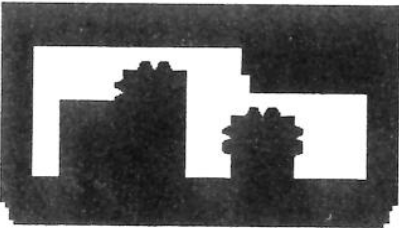
\includegraphics[width=4cm]{figs/alami-transit-slice.png}
      };
      
      \node[inner sep=0] at (11.25,4.25) {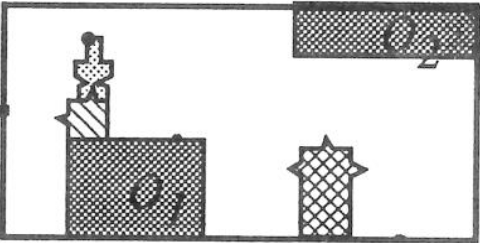
\includegraphics[width=1cm]{figs/alami-transfer-1.png}};
      \node[inner sep=0] at (11.25,3.6) {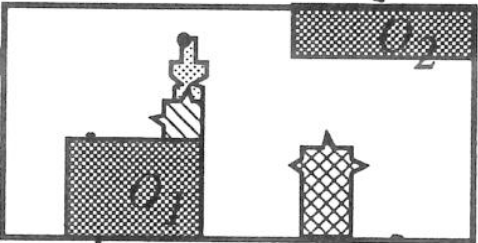
\includegraphics[width=1cm]{figs/alami-intersection.png}};
      \node[inner sep=0] at (11.25,2.95) {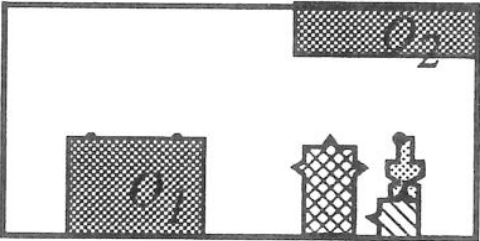
\includegraphics[width=1cm]{figs/alami-transfer-2.png}};
      
      \node at (8.75,4.9) {Transfer Slice:};
      \node[inner sep=0] at (8.5,3.5) {%
         \only<-7>{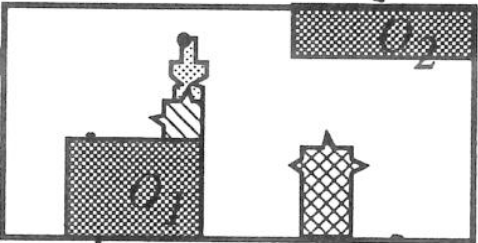
\includegraphics[width=4cm]{figs/alami-intersection.png}}%
         \only<8>{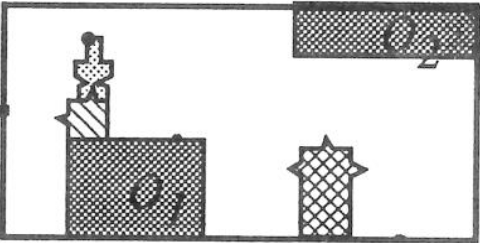
\includegraphics[width=4cm]{figs/alami-transfer-1.png}}%
         \only<9>{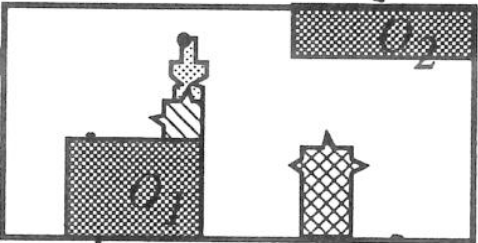
\includegraphics[width=4cm]{figs/alami-intersection.png}}%
         \only<10>{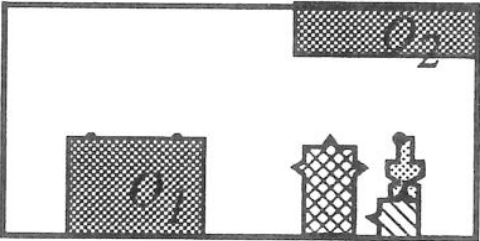
\includegraphics[width=4cm]{figs/alami-transfer-2.png}}%
         \only<11>{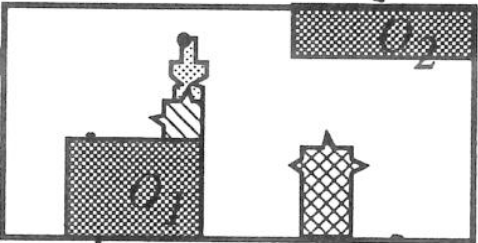
\includegraphics[width=4cm]{figs/alami-intersection.png}}%
      };
      \node[inner sep=0] at (8.5,1.25) {
         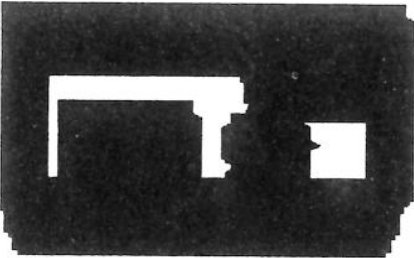
\includegraphics[width=4cm]{figs/alami-transfer-slice.png}
      };
      
   \end{tikzpicture}
\end{frame}

\begin{frame}
   \frametitle{Motivation: 2D Example}
   \begin{tikzpicture}
      \draw[step=1,black!15,very thin,opacity=\gridopacity] (0,0) grid (12,8);
      
      \node[inner sep=0pt] at (6,7) {\begin{minipage}{11.5cm}\centering
         After every grasp and release,
         the projection of the current manifold of $\Pi\mathcal{C}$ onto
         $\mathcal{C}_{\ms{R}}$ changes!
      \end{minipage}};

      \node[inner sep=0] at ( 1.50,5.5) {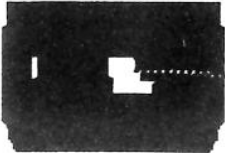
\includegraphics[width=2cm]{figs/alami-slice-01.png}};
      \node[inner sep=0] at ( 3.75,5.5) {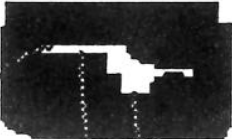
\includegraphics[width=2cm]{figs/alami-slice-02.png}};
      \node[inner sep=0] at ( 6.00,5.5) {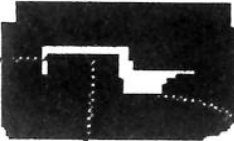
\includegraphics[width=2cm]{figs/alami-slice-03.png}};
      \node[inner sep=0] at ( 8.25,5.5) {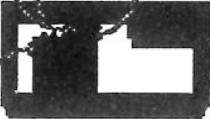
\includegraphics[width=2cm]{figs/alami-slice-04.png}};
      \node[inner sep=0] at (10.50,5.5) {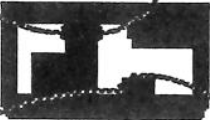
\includegraphics[width=2cm]{figs/alami-slice-05.png}};
      \node[inner sep=0] at ( 1.50,4.0) {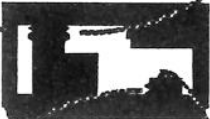
\includegraphics[width=2cm]{figs/alami-slice-06.png}};
      \node[inner sep=0] at ( 3.75,4.0) {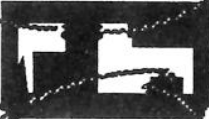
\includegraphics[width=2cm]{figs/alami-slice-07.png}};
      \node[inner sep=0] at ( 6.00,4.0) {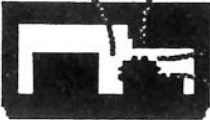
\includegraphics[width=2cm]{figs/alami-slice-08.png}};
      \node[inner sep=0] at ( 8.25,4.0) {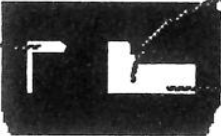
\includegraphics[width=2cm]{figs/alami-slice-09.png}};
      \node[inner sep=0] at (10.50,4.0) {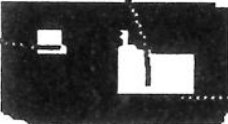
\includegraphics[width=2cm]{figs/alami-slice-10.png}};

      \node[inner sep=0pt] at (6,2.5) {\begin{minipage}{11.5cm}\centering
         Do we need to build a separate roadmap in each slice?
      \end{minipage}};

   \end{tikzpicture}
\end{frame}

\begin{frame}
   \frametitle{Manipulation Example}
   \begin{tikzpicture}
      \draw[step=1,black!15,very thin,opacity=\gridopacity] (0,0) grid (12,8);
      
      \node at (3,6.5) {\includegraphics[width=4.5cm]{build/example-2d-q1}};
      
      \only<3->{
         \node[inner sep=0pt] at (9,7) {\begin{minipage}{5.5cm}\centering
            Query C-Space Subsets:
            
            $S_{12} \subseteq \mathcal{C}$
            
            $S_{23} \subseteq \mathcal{C}$
         \end{minipage}};
      }
      
      \only<3>{
         \node at (9,5.25) {\includegraphics[width=4.5cm]{build/example-2d-s12}};
      }
      \only<4->{
         \node at (9,5.25) {\includegraphics[width=4.5cm]{build/example-2d-s12-wtraj}};
      }
      
      \only<5->{
         \node at (3,4) {\includegraphics[width=4.5cm]{build/example-2d-b}};
      }
      
      \only<6>{
         \node at (9,2.75) {\includegraphics[width=4.5cm]{build/example-2d-s23}};
      }
      \only<7->{
         \node at (9,2.75) {\includegraphics[width=4.5cm]{build/example-2d-s23-wtraj}};
      }
      
      \only<2->{
         \node at (3,1.5) {\includegraphics[width=4.5cm]{build/example-2d-q3}};
      }

   \end{tikzpicture}
\end{frame}

\begin{frame}
   \frametitle{Manipulation Example}
   \begin{tikzpicture}
      \draw[step=1,black!15,very thin,opacity=\gridopacity] (0,0) grid (12,8);
      
      \node at (3,6.5) {\includegraphics[width=4.5cm]{build/example-2d-q1}};
      \node at (3,4) {\includegraphics[width=4.5cm]{build/example-2d-b}};
      \node at (3,1.5) {\includegraphics[width=4.5cm]{build/example-2d-q3}};
      
      \node at (9,4) {\includegraphics{build/figstar-a-qlabeled}};
      
   \end{tikzpicture}
\end{frame}

\begin{frame}
   \frametitle{Workspace Decompositions to C-Space Relations}
   \begin{tikzpicture}
      \draw[step=1,black!15,very thin,opacity=\gridopacity] (0,0) grid (12,8);

      \node[draw,align=center] at (2,6.75) {Workspace\\obstacle\\$W_X$};
      \draw[->,line width=1pt] (3.25,6.75) -- (4.25,6.75);
      \node[align=center] at (6,6.75) {C-Space\\Transforms};
      \draw[->,line width=1pt] (7.75,6.75) -- (8.75,6.75);
      \node[draw,align=center] at (10,6.75) {Valid (free)\\$\mathcal{C}$-subset\\$S_X$};

      % procedure itself
      \only<2->{
         \node[fill=blue!20,rounded corners,anchor=north] at (6,5.5) {\begin{minipage}{5cm}\small{
            {\bf C-Space Set Union Property}$^\dag$
            
            {\bf If} $W_A = W_B \cup W_C$,
            
            {\bf Then} $S_A = S_B \cap S_C$.
         }\end{minipage}};
      
         \node[inner sep=0pt] at (6,0.5) {\begin{minipage}{10.5cm}\scriptsize{
            $^\dag$\PaperPortrait\;  W. S. Newman and M. S. Branicky.
            ``Real-time configuration space transforms for obstacle avoidance.''
            The International Journal of Robotics Research, 1991.
         }\end{minipage}};
      }
      
      \only<3->{
         \node[fill=blue!20,rounded corners,anchor=north] at (6,3.5) {\begin{minipage}{7cm}\small{
            {\bf Example Workspace Decomposition}
            
            {\bf Given} $W_{12}$ {\bf and} $W_{23}$,
            
            {\bf Compute any} $W_C \subseteq W_{12} \cap W_{23}$
            
            {\bf Let} $W_A = W_{12} \setminus W_I$ {\bf and} $W_B = W_{23} \setminus W_I$
            
            {\bf Then} $S_{12} = S_C \cap S_A$ {\bf and} $S_{23} = S_C \cap S_B$
            
         }\end{minipage}};
      }

   \end{tikzpicture}
\end{frame}

\begin{frame}
   \frametitle{Manipulation Example}
   \begin{tikzpicture}
      \draw[step=1,black!15,very thin,opacity=\gridopacity] (0,0) grid (12,8);
      
      \node[font=\small,anchor=east] at (5.25,6.25) {${\hat p}_{12}(q) = 6$};
      \node at (3,5.25) {\includegraphics[width=4.5cm]{build/example-2d-s12}};
      \node[font=\small,anchor=east] at (5.25,3.75) {${\hat p}_{23}(q) = 6$};
      \node at (3,2.75) {\includegraphics[width=4.5cm]{build/example-2d-s23}};
      
      
      \only<3->{
         \node[font=\small,anchor=east] at (11.25,7.5) {${\hat p}_A(q) = 2$};
         \node at (9,6.5) {\includegraphics[width=4.5cm]{build/example-2d-sa}};
      }
      \only<2->{
         \node[font=\small,anchor=east] at (11.25,5.0) {${\hat p}_C(q) = 4$};
         \node at (9,4.0) {\includegraphics[width=4.5cm]{build/example-2d-sc}};
      }
      \only<4->{
         \node[font=\small,anchor=east] at (11.25,2.5) {${\hat p}_B(q) = 2$};
         \node at (9,1.5) {\includegraphics[width=4.5cm]{build/example-2d-sb}};
      }
      
   \end{tikzpicture}
\end{frame}

\begin{frame}
   \frametitle{Manipulation Example}
   \begin{tikzpicture}
      \draw[step=1,black!15,very thin,opacity=\gridopacity] (0,0) grid (12,8);

      \only<1-2>{\node at (9,3.5) {\includegraphics{build/figstar-wo-abc}};}
      
      % left
      \only<1>{
         \node[font=\small,anchor=east] at (5.25,6.25) {${\hat p}_{12}(q) = 6$};
         \node at (3,5.25) {\includegraphics[width=4.5cm]{build/example-2d-s12}};
         \node[font=\small,anchor=east] at (5.25,3.75) {${\hat p}_{23}(q) = 6$};
         \node at (3,2.75) {\includegraphics[width=4.5cm]{build/example-2d-s23}};
      }
      \only<2-3>{
      
         \node[inner sep=0pt] at (3,7.35) {\begin{minipage}{6cm}\centering\small
            $W_{12} = W_C \cup W_A$
            
            $W_{23} = W_C \cup W_B$
         \end{minipage}};
      
         \node[font=\small,anchor=east] at (5.25,6.50) {${\hat p}_A(q) = 2$};
         \node at (3,5.50) {\includegraphics[width=4.5cm]{build/example-2d-sa}};
         \node[font=\small,anchor=east] at (5.25,4.25) {${\hat p}_C(q) = 4$};
         \node at (3,3.25) {\includegraphics[width=4.5cm]{build/example-2d-sc}};
         \node[font=\small,anchor=east] at (5.25,2.00) {${\hat p}_B(q) = 2$};
         \node at (3,1.00) {\includegraphics[width=4.5cm]{build/example-2d-sb}};
      }
      
      % right
      \only<3->{
         \node[inner sep=0pt] at (9,6.75) {\begin{minipage}{6cm}\centering\small
            $S_{12} = S_C \cap S_A$
            
            $S_{23} = S_C \cap S_B$
         \end{minipage}};
      
         \only<3>{\node at (9,3.5) {\includegraphics{build/figstar-w-abc}};}
         \only<4>{\node at (9,3.5) {\includegraphics{build/figstar-traj1}};}
         \only<5>{\node at (9,3.5) {\includegraphics{build/figstar-traj1-inc}};}
      }
      
      % left again
      \only<4->{
         \node at (3,5.25) {\includegraphics[width=4.5cm]{build/example-2d-s12-wtraj}};
      }
      \only<5->{
         \node at (3,2.75) {\includegraphics[width=4.5cm]{build/example-2d-s23-wtraj}};
      }
      
   \end{tikzpicture}
\end{frame}

\begin{frame}
   \frametitle{Multi-Set Planning Formulation}
   \begin{tikzpicture}
      \draw[step=1,black!15,very thin,opacity=\gridopacity] (0,0) grid (12,8);

      % right side
      \node[inner sep=0pt] at (9,6.75) {\begin{minipage}{6cm}\centering\small
            $S_{12} = S_C \cap S_A$
            
            $S_{23} = S_C \cap S_B$
         \end{minipage}};
      \node at (9,3.5) {\includegraphics{build/figstar-w-abc}};
      
      \node[fill=blue!20,rounded corners] at (3,5.5)
      {\begin{minipage}{5cm}
         {\setlength{\tabcolsep}{2pt}
         \begin{tabular}{ccl}
         $\mathcal{C}$ &:& common C-space \\
         \noalign{\medskip}
         $\mathcal{F}$ &:& family of subsets over $\mathcal{C}$ \\
         & & that is, $S \subseteq \mathcal{C} \;\forall\; S \in \mathcal{F}$ \\
         \noalign{\medskip}
         $\mathcal{R}$ &:& set of subset relations \\
         & & e.g. $S_A = S_B \cap S_C$ \\
         \noalign{\medskip}
         $\mathcal{U}$ &:& set of planning queries \\
         & & e.g. $u = (q_{\ms{init}}, q_{\ms{goal}}, S_u)$ \\
         \end{tabular}}
      \end{minipage}};
      
      \node[fill=blue!20,rounded corners] at (3,2)
      {\begin{minipage}{5cm}
         Validity checking model:
         
         {\setlength{\tabcolsep}{2pt}
         \begin{tabular}{ccl}
         ${\bf 1}_A(\cdot)$ &:& indicator for $S_A$ \\
         $p_A(\cdot)$ &:& cost to evaluate ${\bf 1}_A(\cdot)$ \\
         \end{tabular}}
      \end{minipage}};
      
   \end{tikzpicture}
\end{frame}

\begin{frame}
   \frametitle{Instances of Multi-Set Problems in Manipulation}
   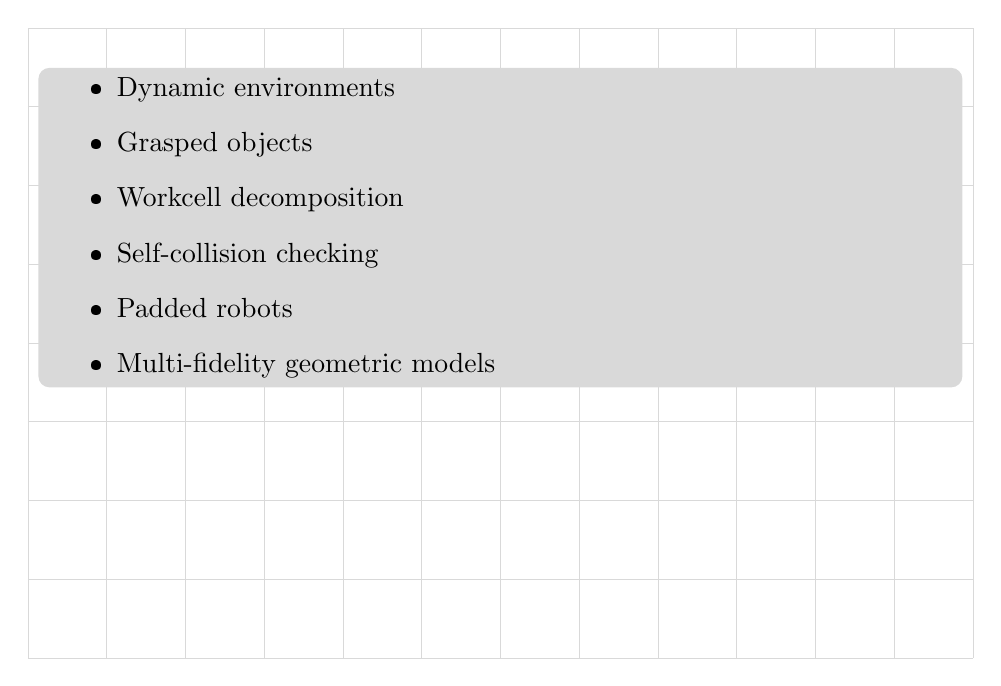
\begin{tikzpicture}
      \draw[step=1,black!15,very thin,opacity=\gridopacity] (0,0) grid (12,8);
      
      \node[anchor=north,fill=black!15,rounded corners]
      at (6,7.5) {\begin{minipage}{11.5cm}
         \begin{itemize}
         \item Dynamic environments
         \item Grasped objects
         \item Workcell decomposition
         \item Self-collision checking
         \item Padded robots
         \item Multi-fidelity geometric models
         \end{itemize}
      \end{minipage}};
   \end{tikzpicture}
\end{frame}

\begin{frame}
   \frametitle{Multi-Set Instances: Dynamic Environments}
   \begin{tikzpicture}
      \draw[step=1,black!15,very thin,opacity=\gridopacity] (0,0) grid (12,8);
      
      \node[inner sep=0pt] at (2.8,4) {%
         \only<1>{\includegraphics[height=7.5cm]{figs/herb-fridge-sets-b.png}}%
         \only<2>{\includegraphics[height=7.5cm]{figs/herb-fridge-sets-a.png}}%
         \only<3>{\includegraphics[height=7.5cm]{figs/herb-fridge-sets-b.png}}%
      };
      
      \node[anchor=north,fill=black!15,rounded corners,font=\small]
      at (8.8,7.75) {\begin{minipage}{6cm}
         The valid set $S_A$ in the presence of an object
         is a subset of the valid set $S_N$ with the object removed.
      \end{minipage}};
      
      \node[inner sep=0pt] at (8.8,4) {%
         \only<1>{\includegraphics[width=4.5cm]{build/multiset-manip-instances,dyna}}%
         \only<2>{\includegraphics[width=4.5cm]{build/multiset-manip-instances,dynb}}%
         \only<3>{\includegraphics[width=4.5cm]{build/multiset-manip-instances,dync}}%
      };
      
   \end{tikzpicture}
\end{frame}

\begin{frame}
   \frametitle{Multi-Set Instances: Dynamic Environments}
   \begin{tikzpicture}
      \draw[step=1,black!15,very thin,opacity=\gridopacity] (0,0) grid (12,8);
      
      \begin{scope}[shift={(1,1.2)},font=\small]
         \node[anchor=south west,inner sep=0] at (0,0)
           {\includegraphics[width=5.2cm]{figs/chimp-voxels-delta.png}};

         \node[draw,inner sep=3pt,fill=white,fill opacity=0.9,align=center]
           (debrislab) at (0.7,1.0) {Debris object\\removed};
         \node[circle,inner sep=2,draw,fill=white] (debris) at (2.2,2.9) {};
         \draw[draw=black, double=white, double distance=1pt, line width=1pt]
           (debrislab.north) -- (debris);
           
         \node[draw,inner sep=3pt,fill=white,fill opacity=0.9,align=center]
           (addlab) at (5.0,2.0) {Additional\\voxels seen};
         \node[circle,inner sep=2,draw,fill=white] (added) at (4.4,5.0) {};
         \draw[draw=black, double=white, double distance=1pt, line width=1pt]
           (addlab.north) -- (added);
      \end{scope}
      
      \node[inner sep=0pt] at (9.5,6) {
         \includegraphics{build/retroactive-a}
      };
      
      \node[inner sep=0pt] at (9.5,2) {
         \includegraphics{build/retroactive-b}
      };
   \end{tikzpicture}
\end{frame}

\begin{frame}
   \frametitle{Multi-Set Instances: Grasped Objects}
   \begin{tikzpicture}
      \draw[step=1,black!15,very thin,opacity=\gridopacity] (0,0) grid (12,8);
      
      \node[inner sep=0pt] at (2.8,4) {%
         \only<1>{\includegraphics[height=7.5cm]{figs/herb-fridge-sets-c.png}}%
         \only<2>{\includegraphics[height=7.5cm]{figs/herb-fridge-sets-a.png}}%
         \only<3>{\includegraphics[height=7.5cm]{figs/herb-fridge-sets-c.png}}%
      };
      
      \node[anchor=north,fill=black!15,rounded corners,font=\small]
      at (8.8,7.75) {\begin{minipage}{6cm}
         The valid set $S_A$ while grasping an object
         is a subset of the valid set $S_N$ with the object removed.
      \end{minipage}};
      
      \node[inner sep=0pt] at (8.8,4) {%
         \only<1>{\includegraphics[width=4.5cm]{build/multiset-manip-instances,dyna}}%
         \only<2>{\includegraphics[width=4.5cm]{build/multiset-manip-instances,dynb}}%
         \only<3>{\includegraphics[width=4.5cm]{build/multiset-manip-instances,dync}}%
      };
      
   \end{tikzpicture}
\end{frame}

\begin{frame}
   \frametitle{Multi-Set Instances: Self-Collision Checking}
   \begin{tikzpicture}
      \draw[step=1,black!15,very thin,opacity=\gridopacity] (0,0) grid (12,8);

      \node[inner sep=0pt] at (2.8,4) {%
         \only<1>{\includegraphics[height=7.5cm]{figs/herb-fridge-sets-a.png}}%
         \only<2>{\includegraphics[height=7.5cm]{figs/herb-fridge-sets-d.png}}%
         \only<3>{\includegraphics[height=7.5cm]{figs/herb-fridge-sets-a.png}}%
      };

      \node[anchor=north,fill=black!15,rounded corners,font=\small]
      at (8.8,7.75) {\begin{minipage}{6cm}
         The valid set $S_A$
         is a subset of the valid set $S_R$
         consisting of robot self-collision-free configurations.
      \end{minipage}};

      \node[inner sep=0pt] at (8.8,4) {%
         \only<1>{\includegraphics[width=4.5cm]{build/multiset-manip-instances,selfa}}%
         \only<2>{\includegraphics[width=4.5cm]{build/multiset-manip-instances,selfb}}%
         \only<3>{\includegraphics[width=4.5cm]{build/multiset-manip-instances,selfc}}%
      };

   \end{tikzpicture}
\end{frame}

\begin{frame}
   \frametitle{Multi-Set Instances: Conservative Obstacle Volumes}
   \begin{tikzpicture}
      \draw[step=1,black!15,very thin,opacity=\gridopacity] (0,0) grid (12,8);
      
      \node[inner sep=0pt] at (2.8,4) {%
         \only<1>{\includegraphics[height=7.5cm]{figs/herb-fridge-sets-h.png}}%
         \only<2-3>{\includegraphics[height=7.5cm]{figs/herb-fridge-sets-e.png}}%
      };
      
      \node[anchor=north,fill=black!15,rounded corners,font=\small]
      at (8.8,7.75) {\begin{minipage}{6cm}
         The valid set $S_O$ in the presence of an object
         can be conservatively bounded by a simpler geometry
         yielding $S_B$.
      \end{minipage}};
      
      \node[inner sep=0pt] at (8.8,4) {%
         \only<1>{\includegraphics[width=4.5cm]{build/multiset-manip-instances-blob,outside}}%
         \only<2->{\includegraphics[width=4.5cm]{build/multiset-manip-instances-blob,inside}}%
      };
      
      \only<3->{
         \node[anchor=north,fill=black!15,rounded corners,font=\small]
         at (8.8,2) {\begin{minipage}{6cm}
            Extreme case: Leven/Hutchinson workcell decomposition.
         \end{minipage}};
      }
      
   \end{tikzpicture}
\end{frame}

\begin{frame}
   \frametitle{Multi-Set Instances: Conservative Grasped Volumes}
   \begin{tikzpicture}
      \draw[step=1,black!15,very thin,opacity=\gridopacity] (0,0) grid (12,8);
      
      \node[inner sep=0pt] at (2.8,4) {%
         \only<1>{\includegraphics[height=7.5cm]{figs/herb-fridge-sets-c.png}}%
         \only<2>{\includegraphics[height=7.5cm]{figs/herb-fridge-sets-i.png}}%
      };
      
      \node[anchor=north,fill=black!15,rounded corners,font=\small]
      at (8.8,7.75) {\begin{minipage}{6cm}
         The valid set $S_O$ while grabbing the object
         can be conservatively bounded by a simpler geometry
         yielding $S_B$.
      \end{minipage}};
      
      \node[inner sep=0pt] at (8.8,4) {%
         \only<1>{\includegraphics[width=4.5cm]{build/multiset-manip-instances-blob,outside}}%
         \only<2>{\includegraphics[width=4.5cm]{build/multiset-manip-instances-blob,inside}}%
      };

   \end{tikzpicture}
\end{frame}

\begin{frame}
   \frametitle{Multi-Set Instances: Conservative Robot Models}
   \begin{tikzpicture}
      \draw[step=1,black!15,very thin,opacity=\gridopacity] (0,0) grid (12,8);
      
      \node[inner sep=0pt] at (2.8,4) {%
         \only<1>{\includegraphics[height=7.5cm]{figs/herb-fridge-sets-j.png}}%
         \only<2->{\includegraphics[height=7.5cm]{figs/herb-fridge-sets-k.png}}%
      };
      
      \node[anchor=north,fill=black!15,rounded corners,font=\small]
      at (8.8,7.75) {\begin{minipage}{6cm}
         The valid set $S_R$ while grabbing the object
         can be conservatively bounded by a simpler geometry
         yielding $S_B$.
      \end{minipage}};
      
      \node[inner sep=0pt] at (8.8,4) {%
         \only<1>{\includegraphics[width=4.5cm]{build/multiset-manip-instances-blob,routside}}%
         \only<2>{\includegraphics[width=4.5cm]{build/multiset-manip-instances-blob,rinside}}%
      };
   
   \end{tikzpicture}
\end{frame}

\begin{frame}
   \frametitle{Instances of Multi-Set Problems in Manipulation}
   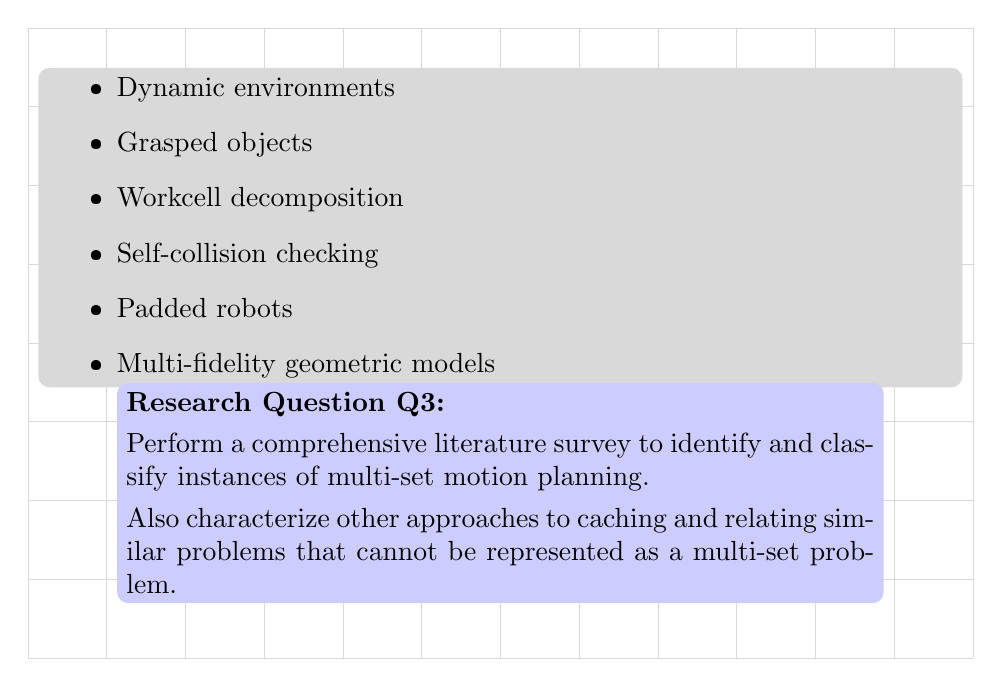
\begin{tikzpicture}
      \draw[step=1,black!15,very thin,opacity=\gridopacity] (0,0) grid (12,8);
      
      \node[anchor=north,fill=black!15,rounded corners]
      at (6,7.5) {\begin{minipage}{11.5cm}
         \begin{itemize}
         \item Dynamic environments
         \item Grasped objects
         \item Workcell decomposition
         \item Self-collision checking
         \item Padded robots
         \item Multi-fidelity geometric models
         \end{itemize}
      \end{minipage}};
      
      \only<2->{
         \node[fill=blue!20,rounded corners,anchor=north]
         at (6,3.5) {\begin{minipage}{9.5cm}
            {\bf Research Question Q3:}
            
            \smallskip
            Perform a comprehensive literature survey to identify
            and classify instances of multi-set motion planning.
            
            \smallskip
            Also characterize other approaches to caching and
            relating similar problems that cannot be represented
            as a multi-set problem.
         \end{minipage}};
      }
      
   \end{tikzpicture}
\end{frame}

\begin{frame}
   \frametitle{Applying the E$^8$-PRM to the Multi-Set Problem}
   \begin{tikzpicture}
      \draw[step=1,black!15,very thin,opacity=\gridopacity] (0,0) grid (12,8);

      \node[fill=blue!20,align=center,rounded corners,
         inner sep=5pt] at (1.5,5.3) {
         Propositional\\
         Logic Solver
      };
      
      \draw[<->,line width=1pt] (2.8,5.3) -- (3.3,5.3);

      \node[shape=document,draw,inner sep=0.25cm,align=center,
         font=\small,anchor=south] at (5,4.5) {
         Multi-Set\\
         ensemble effort\\
         model $\mathcal{M}_{\ms{multi}}$};
      
      \node[anchor=south,shape=document,draw,align=center]
      at (9,4.5) {
         Graph G\\
         \includegraphics[width=2.5cm]{build/roadmap-2d-simple}
         %\includegraphics[width=2.5cm]{build/talk-act1-2d,graph}
         
      };
      
      \draw[->,line width=1pt] (6.3,4.4) -- (6.3,3.9);
      \draw[->,line width=1pt] (7.8,4.4) -- (7.8,3.9);
      
      \node[fill=blue!20,minimum height=1.5cm,minimum width=2.5cm,
         align=center,rounded corners,inner ysep=0.7cm]
      at (7,2.5) {
         E$^8$-PRM\\
         \small{$\min
         \left[ (1 - \lambda) \hat{f}_x + \lambda \hat{f}_p \right]$}
      };
      
      \node[shape=document,draw,align=center,inner xsep=10pt]
      at (2.4,3) {
         Query $V_{s1}$, $V_{g1}$, $\lambda_1$
      };
      \draw[->,line width=1pt] (4.5,3) -- (5.0,3);
      
      \draw[->,line width=1pt] (9,3) -- (9.5,3);
      \node[shape=document,draw,align=center,inner xsep=5pt]
      at (10.1,3) {$\pi^*_1$\;\;};
      
      \node[shape=document,draw,align=center,inner xsep=10pt]
      at (2.4,2) {
         Query $V_{s2}$, $V_{g2}$, $\lambda_2$
      };
      \draw[->,line width=1pt] (4.5,2) -- (5.0,2);
      
      \draw[->,line width=1pt] (9,2) -- (9.5,2);
      \node[shape=document,draw,align=center,inner xsep=5pt]
      at (10.1,2) {$\pi^*_2$\;\;};

      \node[inner sep=0pt] at (6,0.5) {\begin{minipage}{11.5cm}\centering
         This is the Multi-Set PRM.
      \end{minipage}};

   \end{tikzpicture}
\end{frame}

\begin{frame}
   \frametitle{Multi-Set Reasoning with Propositional Logic}
   \begin{tikzpicture}
      \draw[step=1,black!15,very thin,opacity=\gridopacity] (0,0) grid (12,8);

      \node[inner sep=0pt] at (5,6.15) {%
         \only<1>{\includegraphics[width=4.5cm]{build/multiset-roadmap-example,start}}%
         \only<2>{\includegraphics[width=4.5cm]{build/multiset-roadmap-example,roadmap}}%
         \only<3>{\includegraphics[width=4.5cm]{build/multiset-roadmap-example,straightsol}}%
         \only<4-5>{\includegraphics[width=4.5cm]{build/multiset-roadmap-example,basesets}}%
         \only<6>{\includegraphics[width=4.5cm]{build/multiset-roadmap-example,blackgraph}}%
         \only<7>{\includegraphics[width=4.5cm]{build/multiset-roadmap-example,rightsol}}%
         \only<8>{\includegraphics[width=4.5cm]{build/multiset-roadmap-example,leftspec}}%
         \only<9>{\includegraphics[width=4.5cm]{build/multiset-roadmap-example,leftsol}}%
      };
      
      \node[font=\scriptsize,anchor=west] at (7.7,7) {%
         ${\hat p}_u = 2$%
         \only<5->{, \; ${\hat p}_A = {\hat p}_B = 1$}
      };
      
      \only<2->{
         \draw[dotted] (7.7,6.5) -- (8.2,6.5);
         \fill (7.7,6.5) circle (0.04cm);
         \fill (8.2,6.5) circle (0.04cm);
         \node[font=\scriptsize,anchor=west] at (8.3,6.5) {unknown};
      }
      
      \only<3->{
         \draw[color=black!20,line width=5,line cap=round] (7.7,6) -- (8.2,6);
         \node[font=\scriptsize,anchor=west] at (8.3,6) {candidate path ${\hat \pi}^*$};
      }
      
      \only<4->{
         \node[font=\scriptsize,anchor=west] at (7.7,5.5) {$S_u = S_A \cap S_B$};
      }
      
      \only<6->{
         \draw (7.7,5) -- (8.2,5);
         \fill (7.7,5) circle (0.04cm);
         \fill (8.2,5) circle (0.04cm);
         \node[font=\scriptsize,anchor=west] at (8.3,5) {known in $S_A$};
      }
      
      \node[fill=blue!20,rounded corners,font=\scriptsize] at (5,2.1)
      {\begin{minipage}{8cm}
         \begin{algorithmic}[1]
         \Function {MultiOptCert}{$q_e, S_u, P_{\ms{known}}$}
            \State $\mathcal{T}_{\ms{imply}} \leftarrow \emptyset$
            \ForAll {$\mathcal{F}_{\ms{cert}} \in \mathcal{P}(\mathcal{F})$}
                  \label{line:power-set}
               \State ${\hat p}_{\ms{cert}} \leftarrow \sum_{S \in \mathcal{F}_{\ms{cert}}} \hat{p}_S[q_e]$
               \ForAll {$b_{\ms{res}} \mbox{ \textbf{s.t.} }
                     b_{\ms{res}} : \mathcal{F}_{\ms{cert}} \rightarrow \{\mbox{True},\mbox{False}\}$}
                     \label{line:all-binary-functions}
                  \State $\arraycolsep=2pt
                     P_{\ms{res}} \leftarrow
                     \left\{\left. \begin{array}{rl}
                     \mathbf{1}_S & \mbox{if } b_{\ms{res}}(S) \\
                     \lnot \mathbf{1}_S & \mbox{otherwise} \\
                     \end{array}
                     \right|
                     S \in \mathcal{F}_{\ms{cert}}
                     \right\}$
                  \If {$P_{\ms{known}} \cup P_{\ms{res}}
                        \Rightarrow \mathbf{1}_u$ is valid}
                     \State $\mathcal{T}_{\ms{imply}} \leftarrow
                        \mathcal{T}_{\ms{imply}} \cup
                        \{ (\mathcal{F}_{\ms{cert}}, b_{\ms{res}}, {\hat p}_{\ms{cert}}) \}$
                  \EndIf
               \EndFor
            \EndFor
            \State \Return $(\mathcal{F}_{\ms{cert}}, b_{\ms{res}}, {\hat p}_{\ms{cert}})
               \in \mathcal{T}_{\ms{imply}}$
               with lowest ${\hat p}_{\ms{cert}}$
         \EndFunction
         \end{algorithmic}
      \end{minipage}};
      
      \draw[->,line width=1pt] (9.3,2.1) -- (9.8,2.1);
      \node[draw,shape=document,align=center,font=\scriptsize,minimum height=2cm]
         at (10.9,2.1) {Optimistic\\Edge\\Certificate};
      
   \end{tikzpicture}
\end{frame}

\begin{frame}
   \frametitle{Multi-Set PRM Complexity in the Number of Subsets}
   \begin{tikzpicture}
      \draw[step=1,black!15,very thin,opacity=\gridopacity] (0,0) grid (12,8);
   
      \node[fill=blue!20,rounded corners,font=\scriptsize] at (5,5.6)
      {\begin{minipage}{8cm}
         \begin{algorithmic}[1]
         \Function {MultiOptCert}{$q_e, S_u, P_{\ms{known}}$}
            \State $\mathcal{T}_{\ms{imply}} \leftarrow \emptyset$
            \ForAll {$\mathcal{F}_{\ms{cert}} \in \mathcal{P}(\mathcal{F})$}
                  \label{line:power-set}
               \State ${\hat p}_{\ms{cert}} \leftarrow \sum_{S \in \mathcal{F}_{\ms{cert}}} \hat{p}_S[q_e]$
               \ForAll {$b_{\ms{res}} \mbox{ \textbf{s.t.} }
                     b_{\ms{res}} : \mathcal{F}_{\ms{cert}} \rightarrow \{\mbox{True},\mbox{False}\}$}
                     \label{line:all-binary-functions}
                  \State $\arraycolsep=2pt
                     P_{\ms{res}} \leftarrow
                     \left\{\left. \begin{array}{rl}
                     \mathbf{1}_S & \mbox{if } b_{\ms{res}}(S) \\
                     \lnot \mathbf{1}_S & \mbox{otherwise} \\
                     \end{array}
                     \right|
                     S \in \mathcal{F}_{\ms{cert}}
                     \right\}$
                  \If {$P_{\ms{known}} \cup P_{\ms{res}}
                        \Rightarrow \mathbf{1}_u$ is valid}
                     \State $\mathcal{T}_{\ms{imply}} \leftarrow
                        \mathcal{T}_{\ms{imply}} \cup
                        \{ (\mathcal{F}_{\ms{cert}}, b_{\ms{res}}, {\hat p}_{\ms{cert}}) \}$
                  \EndIf
               \EndFor
            \EndFor
            \State \Return $(\mathcal{F}_{\ms{cert}}, b_{\ms{res}}, {\hat p}_{\ms{cert}})
               \in \mathcal{T}_{\ms{imply}}$
               with lowest ${\hat p}_{\ms{cert}}$
         \EndFunction
         \end{algorithmic}
      \end{minipage}};
      
      \draw[->,line width=1pt] (9.3,5.5) -- (9.8,5.5);
      \node[draw,shape=document,align=center,font=\scriptsize,minimum height=2cm]
         at (10.9,5.5) {Optimistic\\Edge\\Certificate};
   
      \only<2->{
         \node[fill=blue!20,rounded corners,anchor=north]
         at (6,3.2) {\begin{minipage}{10.5cm}
            {\bf Research Question Q4:}
            
            \smallskip
            How should the planner manage the potential explosion
            of known subsets over its lifetime?
            
            \smallskip
            Ideas: limiting roadmap depth,
            periodically force-evaluating and/or pruning old subsets
            
         \end{minipage}};
      }
   
   %Talk about failure modes!
   %This is a research question.
   %Complexity, triple-exponential in number of sets?
   
   \end{tikzpicture}
\end{frame}

\begin{frame}
   \frametitle{Multi-Set PRM Behavior: Conservative Volumes}
   \begin{tikzpicture}
      \draw[step=1,black!15,very thin,opacity=\gridopacity] (0,0) grid (12,8);
   
      \node[draw,color=black!25,inner sep=1pt] (lambda0) at (3,6) {%
         \only<1>{\includegraphics[width=5cm]{figs/bean-allpaths-lambda0.png}}%
         \only<2-3>{\includegraphics[width=5cm]{figs/bean-allpaths-padded-lambda0.png}}%
      };
      \node[font=\small,below left=0cm of lambda0.north east] {$\lambda = 0$};
      
      \node[draw,color=black!25,inner sep=1pt] (lambda1) at (3,2) {%
         \only<1-2>{\includegraphics[width=5cm]{figs/bean-allpaths-lambda1.png}}%
         \only<3>{\includegraphics[width=5cm]{figs/bean-allpaths-padded-lambda1.png}}%
      };
      \node[font=\small,below left=0cm of lambda1.north east] {$\lambda = 1$};
      
      \begin{scope}[shift={(7.5,2.5)},font=\small]
      \begin{axis}[
         xlabel=Collision Checks,
         ylabel=Path Length,
         ylabel near ticks,
         xlabel near ticks,
         scaled x ticks=base 10:-3,
         scaled y ticks=base 10:-2,
         every x tick scale label/.style={
            at={(1,-0.2075)}
         },
         %ticks=none,
         axis lines=left,
         xmin=0,xmax=8000,
         ymin=700,ymax=950,
         width=5.5cm, height=5.5cm]
      
      \coordinate (l0) at (axis cs:7219.5, 733.0);
      \coordinate (l1) at (axis cs:4692.6, 836.5);
      \coordinate (l0pad) at (axis cs:2685.7, 733.0);
      \coordinate (l1pad) at (axis cs:1064.5, 907.1);

      \addplot[mark=*] plot coordinates { (7219.5, 733.0) };
      \addplot[mark=*] plot coordinates { (4692.6, 836.5) };

      \node (labl0) at ($ (l0) + (-10,20) $) {$\lambda=0$};
      \node (labl1) at ($ (l1) + (70,20) $) {$\lambda=1$};
      %\draw[->] (labl0) -- ($ (l0)!0.25cm!(labl0) $);
      %\draw[->] (labl1) -- ($ (l1)!0.25cm!(labl1) $);

      % padded nodes
      \only<2-3>{
         \addplot[mark=*] plot coordinates { (2685.7, 733.0) };
         \draw[->,line width=1pt] ($ (l0)!0.15cm!(l0pad) $) -- ($ (l0pad)!0.15cm!(l0) $);
      }
      \only<3>{
         \addplot[mark=*] plot coordinates { (1064.5, 907.1) };
         \draw[->,line width=1pt] ($ (l1)!0.15cm!(l1pad) $) -- ($ (l1pad)!0.15cm!(l1) $);
      }
      
      \end{axis}
      \end{scope}
   
   \end{tikzpicture}
\end{frame}

\begin{frame}
   \frametitle{HERB Example Problem}
   \begin{tikzpicture}
      \draw[step=1,black!15,very thin,opacity=\gridopacity] (0,0) grid (12,8);
   
      \node[inner sep=0pt]
         at ( 1.50,6.6) {\includegraphics[width=2cm]{figs/testherb-a.png}};
      \node[inner sep=0pt]
         at ( 3.75,6.6) {\includegraphics[width=2cm]{figs/testherb-b.png}};
      \node[inner sep=0pt]
         at ( 6.00,6.6) {\includegraphics[width=2cm]{figs/testherb-c.png}};
      \node[inner sep=0pt]
         at ( 8.25,6.6) {\includegraphics[width=2cm]{figs/testherb-d.png}};
      \node[inner sep=0pt]
         at (10.50,6.6) {\includegraphics[width=2cm]{figs/testherb-e.png}};

      \node[inner sep=0pt]
         at ( 2,3.6) {\includegraphics[width=3.9cm]{build/herb-mugbin-plot-1}};
      \node[inner sep=0pt]
         at ( 6,3.6) {\includegraphics[width=3.9cm]{build/herb-mugbin-plot-2}};
      \node[inner sep=0pt]
         at ( 10,3.6) {\includegraphics[width=3.9cm]{build/herb-mugbin-plot-3}};
   
      \only<2->{
         \node[fill=blue!20,rounded corners,anchor=north]
         at (6,1.7) {\begin{minipage}{10.5cm}
            {\bf Research Question Q5:}\\
            Extend experimental evaluation to (a) more problem instances,
            (b) more platforms, (c) more baseline approaches.
         \end{minipage}};
      }
   
   \end{tikzpicture}
\end{frame}

\begin{frame}
   \frametitle{Part 2: Reusing Computation Between Steps}
   \begin{tikzpicture}
      \draw[step=1,black!15,very thin,opacity=\gridopacity] (0,0) grid (12,8);
   
      % figure adapted from proposal doc
      \begin{scope}[font=\scriptsize,shift={(1.5,6.25)}]
         
         % root sets
         \node[draw,black,rounded corners,minimum height=1.5cm,minimum width=0.7cm]
            (Xgrasp) at (3,0) {};
         \node[above=0cm of Xgrasp] {Grasp};
         \node[draw,black,rounded corners,minimum height=1.5cm,minimum width=0.7cm]
            (Xdrop) at (6,0) {};
         \node[above=0cm of Xdrop] {Place};
         
         % nodes
         \node[circle,fill=black,inner sep=2] (xstart) at (0,0) {};
         \node[above=0.1cm of xstart] {$q_{\mbox{\scriptsize start}}$};
         
         % grasp choices
         \node[circle,fill=black,inner sep=2] (xg1) at (2.8,0.5) {};
         \node[circle,fill=black,inner sep=2] (xg2) at (3.1,0.1) {};
         \node[circle,fill=black,inner sep=2] (xg3) at (2.9,-0.5) {};
         % place choices
         \node[circle,fill=black,inner sep=2] (xd1) at (5.9,0.3) {};
         \node[circle,fill=black,inner sep=2] (xd2) at (6.0,-0.4) {};
         % xend 
         \node[circle,fill=black,inner sep=2] (xend) at (9,0) {};
         \node[above=0.1cm of xend] {$q_{\mbox{\scriptsize end}}$};
         
         \draw[line width=1.5mm,white]
            (xstart) .. controls (1,0.2) and (1.4,0.9) .. (xg1);
         \draw[line width=1.5mm,white]
            (xstart) .. controls (1.5,0.2) .. (xg2);
         \draw[line width=1.5mm,white]
            (xstart) .. controls (1.8,-0.6) and (1.6,-0.8) .. (xg3);
         \draw
            (xstart) .. controls (1,0.2) and (1.4,0.9) .. (xg1);
         \draw
            (xstart) .. controls (1.5,0.2) .. (xg2);
         \draw
            (xstart) .. controls (1.8,-0.6) and (1.6,-0.8) .. (xg3);
         \draw[line width=1.5mm,white]
            (xg1) -- (4.7,0.6);
         \draw
            (xg1) -- (4.7,0.6);
         \draw[line width=1.5mm,white]
            (xg2) .. controls (4.5,1) and (3.5,-1.2) .. (4.5,-0.4)
                  .. controls (5.5,0.5) and (5.0,-1.3) .. (xd2);
         \draw
            (xg2) .. controls (4.5,1) and (3.5,-1.2) .. (4.5,-0.4)
                  .. controls (5.5,0.5) and (5.0,-1.3) .. (xd2);
         \draw[line width=1.5mm,white]
            (xg3) .. controls (4.3, 0.2) and (4.5,-0.2) .. (xd1);
         \draw
            (xg3) .. controls (4.3, 0.2) and (4.5,-0.2) .. (xd1);
         % in s3
         \draw[line width=1.5mm,white]
            (xd1) .. controls (8,0.3) and (8,0.1) .. (xend);
         \draw
            (xd1) .. controls (8,0.3) and (8,0.1) .. (xend);
         
         \node[fill,black,rounded corners,minimum height=1.5cm,minimum width=0.7cm,
            opacity=0.1] at (3,0) {};
         \node[fill,black,rounded corners,minimum height=1.5cm,minimum width=0.7cm,
            opacity=0.1] at (6,0) {};
         
      \end{scope}
   
      \fill[green!20] (0.1,3.1) rectangle (11.9,3.7);
   
      \node[anchor=north] at (6,5) {\begin{minipage}{11.5cm}
         Planning for manipulation tasks poses three challenges:
         
         \begin{itemize}
         \item Challenge 1: Capturing the planning/execution tradeoff..
         \item Challenge 2: Incongruent steps impede reuse.
         \item Challenge 3: Coupled steps require long planning horizons.
         \end{itemize}
      \end{minipage}};
   
   \end{tikzpicture}
\end{frame}
